\chapter{Συγγενικές εργασίες}
\label{chap2}

\section{Εισαγωγή}

Εδώ γράφουμε σύντομα τις θεματικές περιοχές στις οποίες έχουμε ανακαλύψει συγγενικές εργασίες, και εξηγούμε γιατί οι περιοχές είναι σχετικές με την διπλωματική. Στη συνέχεια βάζουμε μία υποενότητα για κάθε θεματική περιοχή, όπου και περιγράφουμε σχετικές εργασίες άλλων επιστημόνων.

\section{<Τίτλος για σχετική θεματική περιοχή 1>}

Εδώ περιγράφονται εργασίες που περιγράφουν διαθέσιμες τεχνολογίες/μοντέλα/μεθοδολογίες  στη θεματική περιοχή 1 και είναι σχετικές με την διπλωματική.
Είναι σημαντικό να τονίζουμε τις διαφορές αλλά και τις ομοιότητες σε σχέση με την δική μας διπλωματική. Εφόσον προσθέσετε αυτούσιες εικόνες από άρθρα ή βιβλία τρίτων, θα πρέπει να παραθέσετε την πηγή, όπως στο Σχ. \ref{dataconnection}.

\begin{figure}[t!]
	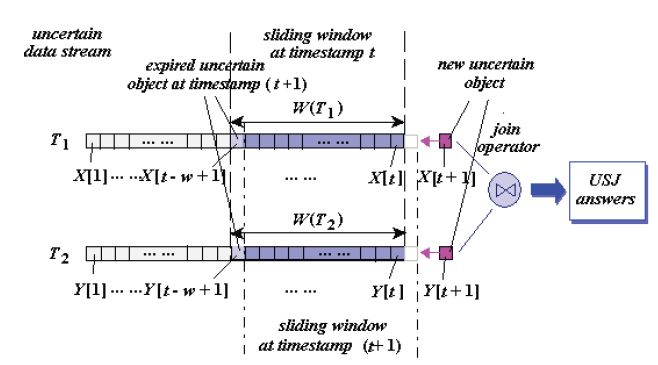
\includegraphics[scale=0.8]{figures/dataconnection.png}
	\centering
	\caption{Παράδειγμα ένταξης εικόνας από άλλο άρθρο ή βιβλίο (Πηγή: \cite{[ACC+03]})}
	\label{dataconnection}
\end{figure}

Στο κείμενό σας, πρέπει να παραθέσετε άρθρα, βιβλία, ιστοσελίδες, άλλες διπλωματικές κλπ. που διαβάσατε. Παραδείγματα παραπομπών:

* από βιβλία: \cite{[RSV02]}

* από άρθρα σε περιοδικά: \cite{[ACC+03],[DRS09],[GBE+00]}

* από άρθρα σε πρακτικά επιστημονικών συνεδρίων: \cite{[JMS+08],[MHP05],[PS11]}

* από ιστοσελίδες: \cite{[Ora11]}

* από διπλωματικές ή άλλες δημοσιευμένες εργασίες: \cite{[Pap15]}


\section{<Τίτλος για σχετική θεματική περιοχή 2>}

Γράψτε το κείμενό σας...

